%beamer

% \newboolean{handoutmode}
% \setboolean{handoutmode}{false}
%\newcommand{\handoutmode}{}

%% LaTeX-Beamer template for KIT design
%% by Erik Burger, Christian Hammer
%% title picture by Klaus Krogmann
%%
%% version 2.1
%%
%% mostly compatible to KIT corporate design v2.0
%% http://intranet.kit.edu/gestaltungsrichtlinien.php
%%
%% Problems, bugs and comments to
%% burger@kit.edu
\ifdefined \handoutmode
\documentclass[18pt, handout]{beamer}
\else
\documentclass[18pt]{beamer}
\fi

\usepackage[T1]{fontenc}
\usepackage[utf8]{inputenc}

\usepackage{../preamble/templates/beamerthemekit}

\usepackage[vlined]{algorithm2e}  %possible: noend, noline, ...
\usepackage{amssymb}
\usepackage{amsmath}
\usepackage{wasysym}
\usepackage{graphicx}
%\usepackage{hyperref}
\usepackage[export]{adjustbox}
\usepackage{wrapfig}
\usepackage{colortbl}
\usepackage{tikz}
\usetikzlibrary{matrix}
\usetikzlibrary{arrows.meta}
\usetikzlibrary{automata}
\usetikzlibrary{tikzmark}
\graphicspath{{images/}}
%\usepackage[colorlinks=true,urlcolor=blue,linkcolor=blue]{hyperref}
\usepackage[outline]{contour}
\usepackage{cancel}
\usepackage[warn]{textcomp}
\usepackage{multicol}
\usepackage{tabularx}
\usepackage{xcolor}
\usepackage{hhline}
\usepackage{environ}
\usepackage{calc}
\usepackage{bm}
\usepackage{xspace} % for \xspace command
\usepackage{varwidth}
\usepackage{csquotes}

\newcommand{\mycomment}[1]{}

%%%% CONFIG

\input{../preamble/config.tex}

%%%% CONFIG END

%\renewcommand{\SS}{\iffontchar\font"1E9E \symbol{"1E9E}\else SS\fi} % SHAME ON YOU, LATEX!
\newcommand{\TM}{\text{$\mbox{}^\text{\tiny TM}$}}
\newcommand{\pluseq}{\mathrel{+}=}
\newcommand{\pp}{\operatorname{++}} 
\newcommand{\mm}{\operatorname{--\mbox{\:}--}}
\newcommand{\minuseq}{\mathrel{-}=}
\newcommand{\asteq}{\mathrel{*}=}
\newcommand{\muleq}{\asteq}
\renewcommand{\mod}{\mathop{\textbf{mod}}} 
\renewcommand{\div}{\mathop{\textbf{div}}}
\newcommand{\N}{\mathbb{N}} 
\newcommand{\R}{\mathbb{R}}
\newcommand{\Z}{\mathbb{Z}}
\newcommand{\E}{\mathbb{E}}
\renewcommand{\P}{\mathbb{P}}
\newcommand{\BB}{\mathbb{B}} % \B already exists
\newcommand{\NP}{\ensuremath{\mathcal{N\hspace{-1.5pt}P}}}
\newcommand{\Oh}[1]{\mathcal{O}\!\left(#1\right)}
\renewcommand{\O}{\mathcal{O}}
\newcommand{\Om}[1]{\Omega\!\left(#1\right)}
\newcommand{\Th}[1]{\Theta\!\left(#1\right)}

\newcommand{\realTilde}{\textasciitilde\xspace}
\renewcommand{\qedsymbol}{\textcolor{black}{\openbox}}

\newcommand{\size}[1]{\ensuremath{\left\lvert #1 \right\rvert}}
\newcommand{\set}[1]{\left\{#1\right\}}
\newcommand{\tuple}[1]{\left(#1\right)}

\newcommand*{\from}{\colon}

\newcommand{\morescalingdelimiters}{   % for proper \left( \right) typography
	\delimitershortfall=0pt  % formerly: 0pt  
	\delimiterfactor=1
}
% todo later
%\delimitershortfall=0pt  % for proper \left( \right) typography
%\delimiterfactor=1

% --- \frameheight constant ---
\newlength\fullframeheight
\newlength\framewithtitleheight
\setlength\fullframeheight{.92\textheight}
\setlength\framewithtitleheight{.86\textheight}

\newlength\frameheight
\setlength\frameheight{\fullframeheight}

\let\frametitleentry\relax
\let\oldframetitle\frametitle
\def\frametitle#1{\global\def\frametitleentry{#1}\if\relax\frametitleentry\relax\else\setlength\frameheight{\framewithtitleheight}\fi\oldframetitle{#1}}

% --- \frameheight constant end ---

\def\·{\cdot}
\def\*{\cdot}
\def\<{\langle}
\def\>{\rangle}


\newcommand{\zB}{z.\,B.\@\xspace}
\newcommand{\ZB}{Z.\,B.\@\xspace}

\newcommand{\ceil}[1]{\left\lceil#1\right\rceil}
\newcommand{\floor}[1]{\left\lfloor#1\right\rfloor}
\newcommand{\abs}[1]{\left|#1\right|}
\newcommand{\Matrix}[1]{\begin{pmatrix} #1 \end{pmatrix}}
\newcommand{\braced}[1]{\left\lbrace #1 \right\rbrace}
\newcommand{\llist}[1]{\langle #1 \rangle}
\newcommand{\Mid}{\;\middle|\;}

\let\after\circ

\newcommand{\entspr}{\ensuremath{\mathrel{\hat{=}}}\xspace}

\def\~~>{\ensuremath{\rightsquigarrow}}  % FuCKING FINALLY! :D

% "something" placeholder. Useful for repairing spacing of operator sections, like `\sth = 42`.
\def\sth{\vphantom{.}}

\def\fract#1/#2 {\frac{#1}{#2}}  % ! TRAILING SPACE is CRUCIAL!
\def\dfract#1/#2 {\dfrac{#1}{#2}} % ! Trailing space is crucial!

\newcommand{\tight}[1]{{\renewcommand{\arraystretch}{0.76} #1}}
\newcommand{\stackedtight}[1]{{\renewcommand{\arraystretch}{0.76} \begin{matrix} #1 \end{matrix}} }
\newcommand{\stacked}[1]{\begin{matrix} #1 \end{matrix} }
\newcommand{\casesl}[1]{\delimitershortfall=0pt  \left\lbrace\hspace{-.3\baselineskip}\begin{array}{ll} #1 \end{array}\right.}
\newcommand{\casesr}[1]{\delimitershortfall=0pt  \left.\begin{array}{ll} #1 \end{array}\right\rbrace}
\newcommand{\caseslr}[1]{\delimitershortfall=0pt  \left\lbrace\begin{array}{ll} #1 \end{array}\hspace{-.3\baselineskip}\right\rbrace}

\def\q#1uad{\ifnum#1=0\relax\else\quad\q{\the\numexpr#1-1\relax}uad\fi}
% e.g. \q1uad = \quad, \q2uad = \qquad etc.

\newcommand{\qqquad}{\q3uad}


\def\indentstring{}
\def\§#1{\def\indentstring{#1}#1}
\def\.{{$\hphantom{\text{\indentstring}}$}}


\newcommand{\impl}{\ifmmode\ensuremath{\mskip\thinmuskip\Rightarrow\mskip\thinmuskip}\else$\Rightarrow$\xspace\fi}  
\newcommand{\Impl}{\ifmmode\implies\else$\Longrightarrow$\xspace\fi}

\newcommand{\gdw}{\ifmmode\mskip\thickmuskip\Leftrightarrow\mskip\thickmuskip\else$\Leftrightarrow$\xspace\fi}
\newcommand{\Gdw}{\ifmmode\iff\else$\Longleftrightarrow$\xspace\fi}

\newcommand{\symbitemnegoffset}{\hspace{-.33\baselineskip}}
\newcommand{\implitem}{\item[\impl\symbitemnegoffset]}
\newcommand{\Implitem}{\item[\Impl\symbitemnegoffset]}


\newcommand{\forcenewline}{\mbox{}\\}

\newcommand{\bfalert}[1]{\textbf{\alert{#1}}}
\let\elem\in   % I'm a Haskell freak. Don't judge me. :P


\newenvironment{threealign}{%
	\[
	\begin{array}{r@{\ }c@{\ }l}
}{%
	\end{array}	
	\]
}


\makeatletter
% Provides color if undefined.
\newcommand{\colorprovide}[2]{%
	\@ifundefinedcolor{#1}{\colorlet{#1}{#2}}{}}
\makeatother



%\pgfdeclarelayer{background}
%\pgfdeclarelayer{foreground}
%\pgfsetlayers{background,main,foreground}

\colorprovide{lightred}{red!30}
\colorprovide{lightgreen}{green!40}
\colorprovide{lightyellow}{yellow!50}
\colorprovide{beamerlightred}{lightred}
\colorprovide{beamerlightgreen}{lightgreen}
\colorprovide{beamerlightyellow}{lightyellow}
\colorprovide{fullred}{red!60}
\colorprovide{fullgreen}{green}
\definecolor{darkred}{RGB}{115,48,38}
\definecolor{darkgreen}{RGB}{48,115,38}
\definecolor{darkyellow}{RGB}{100,100,0}

\only<handout:0>{\colorlet{adaptinglightred}{beamerlightred}}
\only<handout:0>{\colorlet{adaptinglightgreen}{beamerlightgreen}}
\only<handout:0>{\colorlet{adaptinglightyellow}{beamerlightyellow}}
\only<beamer:0>{\colorlet{adaptinglightred}{lightred}}
\only<beamer:0>{\colorlet{adaptinglightgreen}{lightgreen}}
\only<beamer:0>{\colorlet{adaptinglightyellow}{lightyellow}}
\only<handout:0>{\colorlet{adaptingred}{lightred}}
\only<beamer:0>{\colorlet{adaptingred}{fullred}}
\only<handout:0>{\colorlet{adaptinggreen}{lightgreen}}
\only<beamer:0>{\colorlet{adaptinggreen}{fullgreen}}

\colorlet{checkgreen}{green!80}
\colorlet{crashred}{fullred}
\colorprovide{myalertcolor}{red}
\colorlet{alertcolor}{myalertcolor}

\definecolor{kwblue}{rgb}{0.3,0.3,1}
\definecolor{strcolor}{RGB}{48,115,38}

\newcommand{\str}[1]{\shorthandoff{"}\textcolor{strcolor}{\text{"{}#1"{}}\shorthandon{"}}}

\newcommand{\gray}[1]{\textcolor{gray}{#1}}

\newcommand{\MyKwSty}[1]{\textcolor{kwblue}{\textbf{#1}}}
\SetKwSty{MyKwSty}

\SetArgSty{textnormal} % to end conditional italics madness

\newcommand{\MyCommentSty}[1]{\emph{\gray{#1}}}
\SetCommentSty{MyCommentSty}

\SetKwComment{Comment}{// }{}

\newcommand{\LComment}[1]{\Comment*[h]{#1}}
\newcommand{\RComment}[1]{\quad \Comment*[h]{#1}}



\SetKwBlock{KwFunc}{function}{}
\SetKwBlock{KwProc}{procedure}{}
\newcommand{\Function}[2]{\KwFunc({#1}){#2}}
\newcommand{\Procedure}[2]{\KwProc({#1}){#2}}
\SetKwBlock{KwEmptyBlock}{}{}
\newcommand{\EmptyBlock}[1]{\KwEmptyBlock(){#1}}

% Binary operator keywords (small surrounding spaces)
\newcommand{\SetKwBin}[2]{
	\expandafter\newcommand\csname #1\endcsname{\ensuremath{\mathbin{\KwSty{#2}}}}	
}
% Relational operator keywords (bigger surrounding spaces)
\newcommand{\SetKwRel}[2]{
	\expandafter\newcommand\csname #1\endcsname{\ensuremath{\mathrel{\KwSty{#2}}}}	
}
% Directive keywords (trailing space)
\newcommand{\SetKwDir}[2]{
	\expandafter\newcommand\csname #1\endcsname{\ensuremath{\mathop{\KwSty{#2}}}}		
}

\DontPrintSemicolon
%\SetKwSwitch{Switch}{Case}{Other}{switch on}{}{}{else}{}{}

%\newcommand{\SwitchCase}[2]{\KwSty{case} #1 \KwOf\EmptyBlock{#2}}
%\newcommand{\case}[2]{#1:\EmptyBlock{#2}}
\SetKwDir{KwAssert}{assert}
\SetKwDir{KwInvariant}{invariant}
\SetKwRel{KwStep}{step}
\SetKwRel{KwDownto}{downto}	
\SetKwDir{KwArrayOf}{array of\,}
\SetKwDir{KwArray}{array}
\let\KwTo\undefined
\SetKwRel{KwTo}{to}
\SetKwRel{KwOf}{of}
\let\KwInput\KwIn
\let\KwIn\undefined
\SetKwRel{KwIn}{in}
\SetKwRel{KwInto}{into}
\SetKwDir{KwNot}{not}
\SetKwRel{KwIs}{is}
\SetKwRel{KwAnd}{and}
\SetKwRel{KwOr}{or}
\SetKwBin{KwMod}{mod}
\SetKwBin{KwDiv}{div}
\SetKwDir{KwContinue}{continue}
\SetKwDir{KwBreak}{break}
\SetKwDir{KwThrow}{throw}
\SetKw{KwTrue}{true}
\SetKw{KwFalse}{false}
\SetKw{KwThis}{this}
\SetKwDir{KwNew}{new}
\SetKwRel{KwFrom}{from}
\SetKwDir{KwFor}{for}
\SetKwDir{KwEach}{each}
\SetKw{KwProcedure}{procedure}
\SetKw{KwMethod}{method}
\SetKw{KwFunction}{function}
\SetKwDir{KwPointerTo}{Pointer to}
\SetKwData{KwList}{List}
\SetKwData{KwSet}{Set}
\newcommand{\Element}{\|Element|}
\newcommand{\KwListOf}{\ensuremath{\mathop{\KwList \KwOf}}} 
\newcommand{\KwSetOf}{\ensuremath{\mathop{\KwSet \KwOf}}} 
\SetKwDir{KwDispose}{dispose}


\def\|#1|{\text{\normalfont #1}}  % | steht für senkrecht (anstatt kursiv wie sonst im math mode)

% proper math typography
\newcommand{\functionto}{\longrightarrow} 
\renewcommand{\geq}{\geqslant}
\renewcommand{\leq}{\leqslant}
\let\oldsubset\subset
\renewcommand{\subset}{\subseteq} % for all idiots out there using subset

\newcommand{\access}{\text{\textrightarrow}} 
\def\->{\access}

\let\oldemptyset\emptyset
\let\emptyset\varnothing % proper emptyset

\newcommand{\stdarraystretch}{1.20}
\renewcommand{\arraystretch}{\stdarraystretch}  % for proper row spacing in tables

\newcommand{\mailto}[1]{\href{mailto:#1}{{\textcolor{blue}{\underline{#1}}}}}
\newcommand{\urlnamed}[2]{\href{#1}{\textcolor{blue}{\underline{#2}}}}
\renewcommand{\url}[1]{\urlnamed{#1}{#1}}

\newcommand{\hanging}{\hangindent=0.7cm}
\newcommand{\indented}{\hanging}

\newcommand{\Pros}{{\huge \protect\textcolor{adaptinggreen}{\protect\contour{black}{\raisebox{-.3pt}{$\protect\textbf{+}$}}}}\xspace}

\newcommand{\Cons}{\hspace{1pt}\protect\scalebox{0.88}[1]{\huge \protect\contour{black}{\protect\textcolor{adaptingred}{\raisebox{-1pt}{$\protect\textbf{--}$}}}}\hspace{1pt}\xspace}

\newcommand{\yop}{\textcolor{checkgreen}{\protect\contour{black}{\protect\textbf{\checked}}}\xspace}
\newcommand{\crash}{\ensuremath{\textcolor{crashred}{\protect\contour{black}{\protect\textbf{\lightning}}}}\xspace}

\newcommand{\YesCellE}[1]{\cellcolor{adaptinggreen} {#1}}
\newcommand{\YesCell}{\YesCellE{\textbf{Ja}}}
\newcommand{\NoCellE}[1]{\cellcolor{adaptingred} {#1}}
\newcommand{\NoCell}{\NoCellE{\textbf{Nein}}}


\newcommand{\TrueQuestion}[1]{
	\TrueQuestionE{#1}{}
}

\newcommand{\YesQuestion}[1]{
	\YesQuestionE{#1}{}
}

\newcommand{\FalseQuestion}[1]{
	\FalseQuestionE{#1}{}
}

\newcommand{\NoQuestion}[1]{
	\NoQuestionE{#1}{}
}

\newcommand{\DependsQuestion}[1]{
	\DependsQuestionE{#1}{}
}

\newcommand{\QuestionVspace}{\vspace{4pt}}
\newcommand{\QuestionParbox}[1]{\begin{varwidth}{.85\linewidth}#1\end{varwidth}}
\newcommand{\ExplanationParbox}[1]{\begin{varwidth}{.99\linewidth}#1\end{varwidth}}
\colorlet{questionlightgray}{gray!23}
\let\defaultfboxrule\fboxrule

% #1: bg color
% #2: fg color short answer
% #3: short answer text
% #4: question
% #5: explanation
\newcommand{\GenericQuestion}[5]{
	\setlength\fboxrule{2pt}
	\only<+|handout:0>{\hspace{-2pt}\fcolorbox{white}{questionlightgray}{\QuestionParbox{#4} \quad\textbf{?}}}
	\visible<+->{\hspace{-2pt}\fcolorbox{white}{#1}{\QuestionParbox{#4} \quad\textbf{\textcolor{#2}{#3}}} \ExplanationParbox{#5}} \\
	\setlength\fboxrule{\defaultfboxrule}
}

% #1: Q text
% #2: Explanation
\newcommand{\TrueQuestionE}[2]{
	\GenericQuestion{adaptinglightgreen}{darkgreen}{Wahr.}{#1}{#2}
}

% #1: Q text
% #2: Explanation
\newcommand{\YesQuestionE}[2]{
	\GenericQuestion{adaptinglightgreen}{darkgreen}{Ja.}{#1}{#2}
}

% #1: Q text
% #2: Explanation
\newcommand{\FalseQuestionE}[2]{
	\GenericQuestion{adaptinglightred}{darkred}{Falsch.}{#1}{#2}
}

% #1: Q text
% #2: Explanation
\newcommand{\NoQuestionE}[2]{
	\GenericQuestion{adaptinglightred}{darkred}{Nein.}{#1}{#2}
}

% #1: Q text
% #2: Explanation
\newcommand{\DependsQuestionE}[2]{
	\GenericQuestion{adaptinglightyellow}{darkyellow}{Je nachdem!}{#1}{#2}
}

\newenvironment{headframe}{\Huge THIS IS AN ERROR. PLEASE CONTACT THE ADMIN OF THIS TEX CODE. (headframe env def failed)}{}
\RenewEnviron{headframe}[1][]{
	\begin{frame}\frametitle{\ }
		\centering 
		\Huge\textbf{\textsc{\BODY} \\
		} 
		\Large {#1}
		\frametitle{\ }
	\end{frame}
}

\newcommand{\sectionheadframe}[2]{
	\section{#1}
	\begin{headframe}[#2]
		#1
	\end{headframe}	
}

\newcommand{\slideThanks}{
	\begin{frame}{Credits}
		%\begin{block}{}
			Vorgänger dieses Foliensatzes wurden erstellt von: \\[1em]
			Christopher Hommel  (urspr. Verfasser)\\
			Daniel Jungkind 
		%\end{block}
	\end{frame}
}

%% SLIDE FORMAT

% use 'beamerthemekit' for standard 4:3 ratio
% for widescreen slides (16:9), use 'beamerthemekitwide'


% \usepackage{../preamble/templates/beamerthemekitwide}

%% TITLE PICTURE

% if a custom picture is to be used on the title page, copy it into the 'logos'
% directory, in the line below, replace 'mypicture' with the 
% filename (without extension) and uncomment the following line
% (picture proportions: 63 : 20 for standard, 169 : 40 for wide
% *.eps format if you use latex+dvips+ps2pdf, 
% *.jpg/*.png/*.pdf if you use pdflatex)
\IfFileExists{images/logo.png}{
	\titleimage{logo}
}{}
\IfFileExists{images/logo.jpg}{
	\titleimage{logo}
}{}

%% TITLE LOGO

% for a custom logo on the front page, copy your file into the 'logos'
% directory, insert the filename in the line below and uncomment it

\titlelogo{empty}

% (*.eps format if you use latex+dvips+ps2pdf,
% *.jpg/*.png/*.pdf if you use pdflatex)

%% TikZ INTEGRATION

% use these packages for PCM symbols and UML classes
% \usepackage{templates/tikzkit}
% \usepackage{templates/tikzuml}

% the presentation starts here


%% Titel einfügen
\newcommand{\titleframe}{\frame{\titlepage}}

\newcounter{weeknum}

\newcounter{tasknum}
\newcounter{subtasknum}
\resetcounteronoverlays{subtasknum}
\resetcounteronoverlays{tasknum}
\let\oldthesubtasknum\thesubtasknum
\def\thesubtasknum{\ifnum\oldthesubtasknum=0\relax\else\alph{subtasknum})\fi}
\def\ThisHasSubtasks{\setcounter{subtasknum}{1337}}
\def\thetasknumminusone{\the\numexpr\thetasknum-1\relax\xspace}
\newcommand{\taskheading}[1]{\ifnum\oldthesubtasknum=1337\relax\setcounter{subtasknum}{1}\else\setcounter{subtasknum}{0}\fi\addtocounter{tasknum}{1}\textbf{Aufgabe \thetasknum\thesubtasknum: #1} \\}
\newcommand{\subtaskheading}[1]{\addtocounter{subtasknum}{1}\textbf{Aufgabe \thetasknum\thesubtasknum: #1} \\}
\newcommand{\solutionheading}{\textbf{Lösung zu Aufgabe \thetasknum\thesubtasknum} \\}

\setbeamertemplate{section in toc}{
	\gray{\inserttocsection} \par	
}
\setbeamertemplate{navigation symbols}{}

\newif\ifprinttableofcontents \printtableofcontentstrue
\def\notableofcontents{\printtableofcontentsfalse}
\let\notoc\notableofcontents

%% Alles starten mit \starttut{X}
\newcommand{\starttut}[1]{\setcounter{weeknum}{#1}\pdfinfo{
		/Author (\myname)
		/Title  (Algorithmen-Tutorium \mytutnumber, Woche \theweeknum)
	}\titleframe
	\ifprinttableofcontents\frame{\frametitle{Inhalt}\tableofcontents}\fi
	\mycomment{
		\AtBeginSection[]{%
			\begin{frame}{Wo sind wir gerade?}
				\tableofcontents[currentsection]
			\end{frame}\addtocounter{framenumber}{-1}
		}
	}	
}


\newcommand{\framePrevEpisode}{
	\begin{headframe}
		\mylasttimestext
	\end{headframe}
}

\newcommand{\lastframetitled}[6]{
	\frame{\frametitle{#6}
		\vspace{-#2\baselineskip}
		\begin{figure}[H]
			\centering
			\LARGE \textbf{\textsc{#5}} \\
			\vspace{.2\baselineskip}
			\includegraphics[#1]{#3}
			\vspace{-10pt}
			\begin{center}
				\small \url{#4} 
			\end{center}
		\end{figure} 
	}
}

% #1 number
% #2 title 
% #3 vspace (positive) without unit (\baselineskip)
\newcommand{\xkcdframe}[3]{
	\lastframetitled{width=.96\textwidth}{#3}{xkcd_#1}{http://xkcd.com/#1}{}{#2}
}

\newcommand{\xkcdframevert}[3]
{
	\lastframetitled{height=.96\frameheight}{#3}{xkcd_#1}{http://xkcd.com/#1}{}{#2}
}

\newif\ifisWS \isWSfalse

\def\semesterWS{\isWStrue}
\def\semesterSS{\isWSfalse}

\semesterSS

\def\semesterstring{\ifisWS WS \thisyear/\the\numexpr\nextyear-2000\relax\else SS \thisyear\fi}

\edef\nextyear{\the\numexpr\thisyear+1\relax} 

\title[Algorithmen-Tutorium \mytutnumber, Woche \theweeknum]{Algorithmen I \\[-2pt] Tutorium \mytutnumber}
\subtitle{Woche \theweeknum\ |\xspace\mydate{\theweeknum}}


\author[\myname]{{\mynamebold \; (\mailto{\mymail})}}

\institute{Institut für Theoretische Informatik}

\date{\mydate{\theweeknum}\ }



% Bibliography
% not needed here:
%\usepackage[citestyle=authoryear,bibstyle=numeric,hyperref,backend=biber]{biblatex}
%\addbibresource{templates/example.bib}
%\bibhang1em

% presentation

\setbeamercovered{transparent=1}  %min=0, max=100

% change the following line to "ngerman" for German style date and logos
\selectlanguage{ngerman}

\ifnum\thisyear=2018 \else \errmessage{Old ILIAS link inside preamble. Please update.} \fi

\newcommand{\ILIAS}{\urlnamed{https://ilias.studium.kit.edu/ilias.php?ref_id=808428&cmdClass=ilrepositorygui&cmdNode=k8&baseClass=ilrepositorygui}{ILIAS}\xspace} 

\newcommand{\Socrative}{\only<handout:0>{socrative.com $\qquad$ \~~> Student login \\ Raumname:  \mysocrativeroom\\ \medskip}}

\newcommand{\thasse}[1]{
	\ifdefined\ThassesTut #1\xspace \else\fi
}
\newcommand{\daniel}[1]{
	\ifdefined\DanielsTut #1\xspace \else\fi
}
\newcommand{\thassedaniel}[2]{\ifdefined\ThassesTut #1\else\ifdefined\DanielsTut #2\fi\fi\xspace}

\ifdefined\ThassesTut \ifdefined\DanielsTut \errmessage{ERROR: Both ThassesTut and DanielsTut flags are set. This is most likely an error. Please check your config.tex file.} \else \fi \else \ifdefined\DanielsTut \else \errmessage{ERROR: Neither ThassesTut  nor DanielsTut flags are set. This is most likely an error. Please check your config.tex file.} \fi\fi

\begin{document}
	
\starttut{6}

\iffalse

\begin{frame}{Zum letzten Übungsblatt}
	\textbf{Achtung bei der Wahl von Datenstrukturen} \\[0,125cm]
	\begin{itemize}
		\pause
		\item Aufgabenstellung spezifiziert nicht, ob eine Menge von Daten als Array oder Liste gegeben ist \impl Beides darf als Parametertyp gewählt werden
		\pause
		\item Aber: Wenn über die Daten iteriert wird, folgendes beachten:
		\pause
		\item Listen bieten Indexzugriff i.A. \textbf{nicht in konstanter Zeit}! D.h. wenn man „via Index“ über eine Liste iteriert, hat die Iteration eine Laufzeit von $\Theta(n^2)$
		\pause
		\item Daher: Iteration bei Arrays frei via Index oder \textit{for-each}, bei Listen \textbf{nur} \textit{for-each}, wenn die Laufzeit wichtig ist (bei Arrays und Listen kann davon ausgegangen werden, dass \textit{for-each} die Daten in linearer Reihenfolge durchläuft)
	\end{itemize}
\end{frame}

\fi

\mycomment{
	\begin{frame}{Zu Blatt \#5}
		Durchschnitt: \quad etwa \thassedaniel{XXX}{XXX}~\% der Punkte
		\begin{itemize}
			\item ...
		\end{itemize}
	\end{frame}
}

\sectionheadframe{Quicksort}{Eine erquickende Neuerung}

\begin{frame}{Quicksort}
	\begin{itemize}
		\item Erinnerung: Array sortierbar durch Einteilung in sortierten und unsortierten Bereich
		\pause
		\implitem \textbf{Idee: „Semi-Sortierung“} \\
		Wähle beliebiges Pivotelement $p$ (in $O(1)$) und teile auf (in $O(n)$):
		\begin{tabular}{|c|c|}
			\hline
			$\qquad \leq p \qquad$  & $\qquad > p \qquad$  \\
			\hline
		\end{tabular} \\
		\forcenewline
		Diese Teile dann rekursiv weitersortieren.
	\end{itemize}
\end{frame}

\begin{frame}{Quicksort – Beispiel}
	Sortiere $A = (5,3,8,4,2,6,1): \KwArray[1..n] \KwOf \N$ mit Quicksort. Wähle als Pivot $p(A) := A[\ceil{\fract n/2 }]$. Zeichne dazu den Rekursionsbaum.
	\visible<2->{
		\begin{center}
			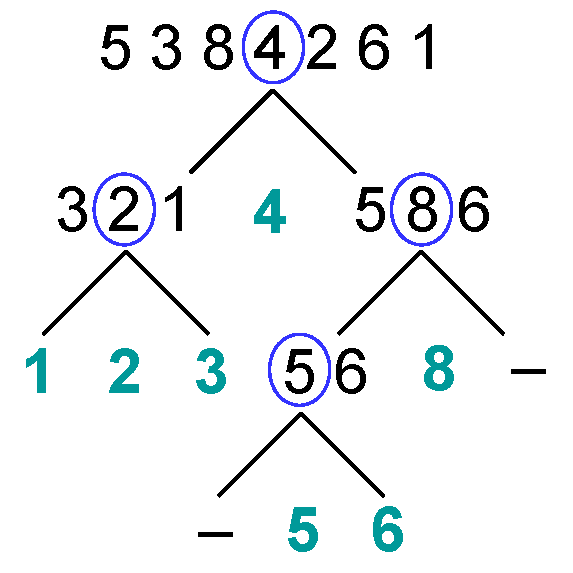
\includegraphics[width=.5\textwidth]{qstree}
		\end{center}	
	}
\end{frame}

\begin{frame}{Quicksort (mit partition)}
	\begin{itemize}
		\item Wie effizient und platzsparend aufteilen? \\
		\impl \textbf{partition}! $O(1)$ Platz und $O(n)$ Zeit  \\
		(Siehe nächste Folien...)
		\pause
		\item \textbf{Laufzeit}: Master-Theorem nicht anwendbar, da Größe der rekursiven Aufrufe \textbf{nicht} in Voraus bekannt
		\pause
		\item Worst-Case $\Theta(n^2)$ möglich
		\pause
		\item Vorlesung sagt: \textbf{Erwartete} Laufzeit in $\Theta(n \log n)$
	\end{itemize}
\end{frame}

\begin{frame}[t]{Quicksort (mit partition)}
	\textbf{Beispiel} \\
	Partitioniere $A: \KwArray[0..n-1]$ mit Pivotwahl $p(A) := A[\floor{\fract n/3 }]$ {\small (mit $n := \abs{A}$)}
	\\[0,5cm]
	\begin{tabular}{ | c | c | c | c | c | c | c | }
		\multicolumn{7}{ c }{ }
		\\ \hline
		1 & 8 & 6 & 9 & 1 & 7 & 0
		\\ \hline
	\end{tabular}\\
	\vspace{3\baselineskip}
	\hyperlink{label:afterEx1}{Hier klicken, um das Beispiel zu überspringen.}
\end{frame}



\begin{frame}[t]{Quicksort (mit partition)}
	\textbf{Beispiel} \\
	Partitioniere $A: \KwArray[0..n-1]$ mit Pivotwahl $p(A) := A[\floor{\fract n/3 }]$ {\small (mit $n := \abs{A}$)}
	\\[0,5cm]
	\begin{tabular}{ | c | c | c | c | c | c | c | }
		\multicolumn{2}{ c| }{ } & p & \multicolumn{4}{ c }{ }
		\\ \hline
		1 & 8 & \cellcolor{yellow} 6 & 9 & 1 & 7 & 0
		\\ \hline
	\end{tabular}
\end{frame}

\begin{frame}[t]{Quicksort (mit partition)}
	\textbf{Beispiel} \\
	Partitioniere $A: \KwArray[0..n-1]$ mit Pivotwahl $p(A) := A[\floor{\fract n/3 }]$ {\small (mit $n := \abs{A}$)}
	\\[0,5cm]
	\begin{tabular}{ | c | c | c | c | c | c | c | }
		\multicolumn{6}{ c| }{ } & p
		\\ \hline
		1 & 8 & 0 & 9 & 1 & 7 & \cellcolor{yellow} 6
		\\ \hline
	\end{tabular}
\end{frame}

\begin{frame}[t]{Quicksort (mit partition)}
	\textbf{Beispiel} \\
	Partitioniere $A: \KwArray[0..n-1]$ mit Pivotwahl $p(A) := A[\floor{\fract n/3 }]$ {\small (mit $n := \abs{A}$)}
	\\[0,5cm]
	\begin{tabular}{ | c | c | c | c | c | c | c | }
		\multicolumn{6}{ c| }{ } & p
		\\ \hline
		\cellcolor{cyan!50} 1 & 8 & 0 & 9 & 1 & 7 & \cellcolor{yellow} 6
		\\ \hline
	\end{tabular}
\end{frame}

\begin{frame}[t]{Quicksort (mit partition)}
	\textbf{Beispiel} \\
	Partitioniere $A: \KwArray[0..n-1]$ mit Pivotwahl $p(A) := A[\floor{\fract n/3 }]$ {\small (mit $n := \abs{A}$)}
	\\[0,5cm]
	\begin{tabular}{ | c | c | c | c | c | c | c | }
		$ \leq p$ & \multicolumn{5}{ c| }{ } & p
		\\ \hline
		\cellcolor{adaptingred} 1 & 8 & 0 & 9 & 1 & 7 & \cellcolor{yellow} 6
		\\ \hline
	\end{tabular}
\end{frame}

\begin{frame}[t]{Quicksort (mit partition)}
	\textbf{Beispiel} \\
	Partitioniere $A: \KwArray[0..n-1]$ mit Pivotwahl $p(A) := A[\floor{\fract n/3 }]$ {\small (mit $n := \abs{A}$)}
	\\[0,5cm]
	\begin{tabular}{ | c | c | c | c | c | c | c | }
		$ \leq p$ & \multicolumn{5}{ c| }{ } & p
		\\ \hline
		\cellcolor{adaptingred} 1 & \cellcolor{cyan!50} 8 & 0 & 9 & 1 & 7 & \cellcolor{yellow} 6
		\\ \hline
	\end{tabular}
\end{frame}

\begin{frame}[t]{Quicksort (mit partition)}
	\textbf{Beispiel} \\
	Partitioniere $A: \KwArray[0..n-1]$ mit Pivotwahl $p(A) := A[\floor{\fract n/3 }]$ {\small (mit $n := \abs{A}$)}
	\\[0,5cm]
	\begin{tabular}{ | c | c | c | c | c | c | c | }
		$ \leq p$ & $ > p$ & \multicolumn{4}{ c| }{ } & p
		\\ \hline
		\cellcolor{adaptingred} 1 & \cellcolor{adaptinggreen} 8 & 0 & 9 & 1 & 7 & \cellcolor{yellow} 6
		\\ \hline
	\end{tabular}
\end{frame}

\begin{frame}[t]{Quicksort (mit partition)}
	\textbf{Beispiel} \\
	Partitioniere $A: \KwArray[0..n-1]$ mit Pivotwahl $p(A) := A[\floor{\fract n/3 }]$ {\small (mit $n := \abs{A}$)}
	\\[0,5cm]
	\begin{tabular}{ | c | c | c | c | c | c | c | }
		$ \leq p$ & $ > p$ & \multicolumn{4}{ c| }{ } & p
		\\ \hline
		\cellcolor{adaptingred} 1 & \cellcolor{adaptinggreen} 8 & \cellcolor{cyan!50} 0 & 9 & 1 & 7 & \cellcolor{yellow} 6
		\\ \hline
	\end{tabular}
\end{frame}

\begin{frame}[t]{Quicksort (mit partition)}
	\textbf{Beispiel} \\
	Partitioniere $A: \KwArray[0..n-1]$ mit Pivotwahl $p(A) := A[\floor{\fract n/3 }]$ {\small (mit $n := \abs{A}$)}
	\\[0,5cm]
	\begin{tabular}{ | c | c | c | c | c | c | c | }
		\multicolumn{2}{ |c| }{$ \leq p$} & $ > p$ & \multicolumn{3}{ c| }{ } & p
		\\ \hline
		\cellcolor{adaptingred} 1 & \cellcolor{adaptingred} 0 & \cellcolor{adaptinggreen} 8 & 9 & 1 & 7 & \cellcolor{yellow} 6
		\\ \hline
	\end{tabular}
\end{frame}

\begin{frame}[t]{Quicksort (mit partition)}
	\textbf{Beispiel} \\
	Partitioniere $A: \KwArray[0..n-1]$ mit Pivotwahl $p(A) := A[\floor{\fract n/3 }]$ {\small (mit $n := \abs{A}$)}
	\\[0,5cm]
	\begin{tabular}{ | c | c | c | c | c | c | c | }
		\multicolumn{2}{ |c| }{$ \leq p$} & $ > p$ & \multicolumn{3}{ c| }{ } & p
		\\ \hline
		\cellcolor{adaptingred} 1 & \cellcolor{adaptingred} 0 & \cellcolor{adaptinggreen} 8 & \cellcolor{cyan!50} 9 & 1 & 7 & \cellcolor{yellow} 6
		\\ \hline
	\end{tabular}
\end{frame}

\begin{frame}[t]{Quicksort (mit partition)}
	\textbf{Beispiel} \\
	Partitioniere $A: \KwArray[0..n-1]$ mit Pivotwahl $p(A) := A[\floor{\fract n/3 }]$ {\small (mit $n := \abs{A}$)}
	\\[0,5cm]
	\begin{tabular}{ | c | c | c | c | c | c | c | }
		\multicolumn{2}{ |c| }{$ \leq p$} & \multicolumn{2}{ c| }{$ > p$} & \multicolumn{2}{ c| }{ } & p
		\\ \hline
		\cellcolor{adaptingred} 1 & \cellcolor{adaptingred} 0 & \cellcolor{adaptinggreen} 8 & \cellcolor{adaptinggreen} 9 & 1 & 7 & \cellcolor{yellow} 6
		\\ \hline
	\end{tabular}
\end{frame}

\begin{frame}[t]{Quicksort (mit partition)}
	\textbf{Beispiel} \\
	Partitioniere $A: \KwArray[0..n-1]$ mit Pivotwahl $p(A) := A[\floor{\fract n/3 }]$ {\small (mit $n := \abs{A}$)}
	\\[0,5cm]
	\begin{tabular}{ | c | c | c | c | c | c | c | }
		\multicolumn{2}{ |c| }{$ \leq p$} & \multicolumn{2}{ c| }{$ > p$} & \multicolumn{2}{ c| }{ } & p
		\\ \hline
		\cellcolor{adaptingred} 1 & \cellcolor{adaptingred} 0 & \cellcolor{adaptinggreen} 8 & \cellcolor{adaptinggreen} 9 & \cellcolor{cyan!50} 1 & 7 & \cellcolor{yellow} 6
		\\ \hline
	\end{tabular}
\end{frame}

\begin{frame}[t]{Quicksort (mit partition)}
	\textbf{Beispiel} \\
	Partitioniere $A: \KwArray[0..n-1]$ mit Pivotwahl $p(A) := A[\floor{\fract n/3 }]$ {\small (mit $n := \abs{A}$)}
	\\[0,5cm]
	\begin{tabular}{ | c | c | c | c | c | c | c | }
		\multicolumn{3}{ |c| }{$ \leq p$} & \multicolumn{2}{ c| }{$ > p$} &  & p
		\\ \hline
		\cellcolor{adaptingred} 1 & \cellcolor{adaptingred} 0 & \cellcolor{adaptingred} 1 & \cellcolor{adaptinggreen} 9 & \cellcolor{adaptinggreen} 8 & 7 & \cellcolor{yellow} 6
		\\ \hline
	\end{tabular}
\end{frame}

\begin{frame}[t]{Quicksort (mit partition)}
	\textbf{Beispiel} \\
	Partitioniere $A: \KwArray[0..n-1]$ mit Pivotwahl $p(A) := A[\floor{\fract n/3 }]$ {\small (mit $n := \abs{A}$)}
	\\[0,5cm]
	\begin{tabular}{ | c | c | c | c | c | c | c | }
		\multicolumn{3}{ |c| }{$ \leq p$} & \multicolumn{2}{ c| }{$ > p$} &  & p
		\\ \hline
		\cellcolor{adaptingred} 1 & \cellcolor{adaptingred} 0 & \cellcolor{adaptingred} 1 & \cellcolor{adaptinggreen} 9 & \cellcolor{adaptinggreen} 8 & \cellcolor{cyan!50} 7 & \cellcolor{yellow} 6
		\\ \hline
	\end{tabular}
\end{frame}

\begin{frame}[t]{Quicksort (mit partition)}
	\textbf{Beispiel} \\
	Partitioniere $A: \KwArray[0..n-1]$ mit Pivotwahl $p(A) := A[\floor{\fract n/3 }]$ {\small (mit $n := \abs{A}$)}
	\\[0,5cm]
	\begin{tabular}{ | c | c | c | c | c | c | c | }
		\multicolumn{3}{ |c| }{$ \leq p$} & \multicolumn{3}{ c| }{$ > p$} & p
		\\ \hline
		\cellcolor{adaptingred} 1 & \cellcolor{adaptingred} 0 & \cellcolor{adaptingred} 1 & \cellcolor{adaptinggreen} 9 & \cellcolor{adaptinggreen} 8 & \cellcolor{adaptinggreen} 7 & \cellcolor{yellow} 6
		\\ \hline
	\end{tabular}
\end{frame}



\begin{frame}[t]{\hypertarget{label:afterEx1}{}Quicksort (mit partition)}
	\textbf{Beispiel} \\
	Partitioniere $A: \KwArray[0..n-1]$ mit Pivotwahl $p(A) := A[\floor{\fract n/3 }]$ {\small (mit $n := \abs{A}$)}
	\\[0,5cm]
	\begin{tabular}{ | c | c | c | c | c | c | c | }
		\multicolumn{3}{ |c| }{$ \leq p$} & p & \multicolumn{3}{ c| }{$ > p$}
		\\ \hline
		\cellcolor{adaptingred} 1 & \cellcolor{adaptingred} 0 & \cellcolor{adaptingred} 1 & \cellcolor{yellow} 6 & \cellcolor{adaptinggreen} 8 & \cellcolor{adaptinggreen} 7 & \cellcolor{adaptinggreen} 9
		\\ \hline
	\end{tabular}
\end{frame}



\begin{frame}{Quicksort (mit partition)}
	\textbf{Schema aus der Vorlesung}
	\begin{figure}[htp]
		\centering
		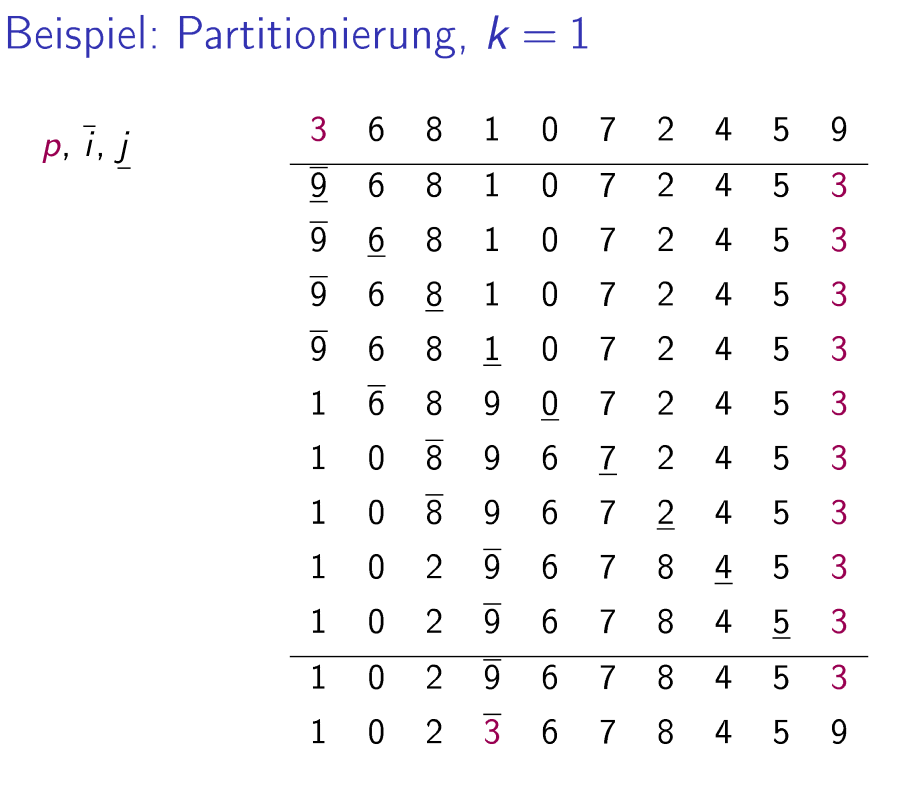
\includegraphics[height=6cm]{quicksortpartition}
	\end{figure}
\end{frame}

\begin{frame}[t]{Quicksort (mit partition)}
	Laufzeit, wenn alle Zahlen gleich sind? \\
	\pause
	\impl $\Theta(n^2)$ \\
	\pause
	\FalseQuestionE{Quicksort (mit partition) ist stabil.}{„Durcheinandermischen“ bei partition macht's kaputt.} 
	\DependsQuestionE{Quicksort ist in-place.}{
		\textbf{Rekursionsaufrufe} benötigen $\Theta( \log n)$ (vernachlässigbar) viel Platz (\impl Stack-Overhead). Abgesehen davon \textbf{kein} weiterer Verwaltungsaufwand.
	}
\end{frame}

\begin{frame}{Quicksort (besseres partition)}
	\textbf{Aller guten Dinge sind drei!} \\
	\begin{itemize}
		\item Worst-Case von eben: schlecht \frownie
		\pause
		\implitem Besser: \textbf{Drei-Wege-Partitionierung}!
		\item Führe einen zusätzlichen Bereich $ = p$ ein: \\
		\begin{tabular}{|c|c|c|}
			\hline
			$\qquad < p \qquad$ & \cellcolor{cyan!50} $\qquad = p \qquad$ & $\qquad > p \qquad$ \\
			\hline
		\end{tabular} 
	\end{itemize}
\end{frame}


\begin{frame}[t]{Quicksort (mit Drei-Wege-Partitionierung)}
	\textbf{Beispiel} \\
	Partitioniere $A: \KwArray[0..n-1]$ mit Pivotwahl $p(A) := A[\floor{\fract n/3 }]$ {\small (mit $n := \abs{A}$)}
	\\[0,5cm]
	\begin{tabular}{ | c | c | c | c | c | c | c | c | c | }
		\multicolumn{9}{ c }{ }
		\\ \hline
		3 & 7 & 0 & 5 & 1 & 5 & 5 & 7 & 1
		\\ \hline
	\end{tabular}\\
	\vspace{3\baselineskip}
	\hyperlink{label:afterEx2}{Hier klicken, um das Beispiel zu überspringen.}
\end{frame}



\begin{frame}[t]{Quicksort (mit Drei-Wege-Partitionierung)}
	\textbf{Beispiel} \\
	Partitioniere $A: \KwArray[0..n-1]$ mit Pivotwahl $p(A) := A[\floor{\fract n/3 }]$ {\small (mit $n := \abs{A}$)}
	\\[0,5cm]
	\begin{tabular}{ | c | c | c | c | c | c | c | c | c | }
		\multicolumn{9}{ c }{ }
		\\ \hline
		3 & 7 & 0 & \cellcolor{yellow} 5 & 1 & 5 & 5 & 7 & 1
		\\ \hline
	\end{tabular}
\end{frame}

\begin{frame}[t]{Quicksort (mit Drei-Wege-Partitionierung)}
	\textbf{Beispiel} \\
	Partitioniere $A: \KwArray[0..n-1]$ mit Pivotwahl $p(A) := A[\floor{\fract n/3 }]$ {\small (mit $n := \abs{A}$)}
	\\[0,5cm]
	\begin{tabular}{ | c | c | c | c | c | c | c | c | c | }
		\multicolumn{8}{ c| }{ } & p
		\\ \hline
		3 & 7 & 0 & 1 & 1 & 5 & 5 & 7 & \cellcolor{yellow} 5
		\\ \hline
	\end{tabular}
\end{frame}

\begin{frame}[t]{Quicksort (mit Drei-Wege-Partitionierung)}
	\textbf{Beispiel} \\
	Partitioniere $A: \KwArray[0..n-1]$ mit Pivotwahl $p(A) := A[\floor{\fract n/3 }]$ {\small (mit $n := \abs{A}$)}
	\\[0,5cm]
	\begin{tabular}{ | c | c | c | c | c | c | c | c | c | }
		\multicolumn{8}{ c| }{ } & p
		\\ \hline
		\cellcolor{cyan!50} 3 & 7 & 0 & 1 & 1 & 5 & 5 & 7 & \cellcolor{yellow} 5
		\\ \hline
	\end{tabular}
\end{frame}

\begin{frame}[t]{Quicksort (mit Drei-Wege-Partitionierung)}
	\textbf{Beispiel} \\
	Partitioniere $A: \KwArray[0..n-1]$ mit Pivotwahl $p(A) := A[\floor{\fract n/3 }]$ {\small (mit $n := \abs{A}$)}
	\\[0,5cm]
	\begin{tabular}{ | c | c | c | c | c | c | c | c | c | }
		$ < p$ & \multicolumn{7}{ c| }{ } & p
		\\ \hline
		\cellcolor{adaptingred} 3 & 7 & 0 & 1 & 1 & 5 & 5 & 7 & \cellcolor{yellow} 5
		\\ \hline
	\end{tabular}
\end{frame}

\begin{frame}[t]{Quicksort (mit Drei-Wege-Partitionierung)}
	\textbf{Beispiel} \\
	Partitioniere $A: \KwArray[0..n-1]$ mit Pivotwahl $p(A) := A[\floor{\fract n/3 }]$ {\small (mit $n := \abs{A}$)}
	\\[0,5cm]
	\begin{tabular}{ | c | c | c | c | c | c | c | c | c | }
		$ < p$ & \multicolumn{7}{ c| }{ } & p
		\\ \hline
		\cellcolor{adaptingred} 3 & \cellcolor{cyan!50} 7 & 0 & 1 & 1 & 5 & 5 & 7 & \cellcolor{yellow} 5
		\\ \hline
	\end{tabular}
\end{frame}

\begin{frame}[t]{Quicksort (mit Drei-Wege-Partitionierung)}
	\textbf{Beispiel} \\
	Partitioniere $A: \KwArray[0..n-1]$ mit Pivotwahl $p(A) := A[\floor{\fract n/3 }]$ {\small (mit $n := \abs{A}$)}
	\\[0,5cm]
	\begin{tabular}{ | c | c | c | c | c | c | c | c | c | }
		$ < p$ & $ > p $ & \multicolumn{6}{ c| }{ } & p
		\\ \hline
		\cellcolor{adaptingred} 3 & \cellcolor{adaptinggreen} 7 & 0 & 1 & 1 & 5 & 5 & 7 & \cellcolor{yellow} 5
		\\ \hline
	\end{tabular}
\end{frame}

\begin{frame}[t]{Quicksort (mit Drei-Wege-Partitionierung)}
	\textbf{Beispiel} \\
	Partitioniere $A: \KwArray[0..n-1]$ mit Pivotwahl $p(A) := A[\floor{\fract n/3 }]$ {\small (mit $n := \abs{A}$)}
	\\[0,5cm]
	\begin{tabular}{ | c | c | c | c | c | c | c | c | c | }
		$ < p$ & $ > p $ & \multicolumn{6}{ c| }{ } & p
		\\ \hline
		\cellcolor{adaptingred} 3 & \cellcolor{adaptinggreen} 7 & \cellcolor{cyan!50} 0 & 1 & 1 & 5 & 5 & 7 & \cellcolor{yellow} 5
		\\ \hline
	\end{tabular}
\end{frame}

\begin{frame}[t]{Quicksort (mit Drei-Wege-Partitionierung)}
	\textbf{Beispiel} \\
	Partitioniere $A: \KwArray[0..n-1]$ mit Pivotwahl $p(A) := A[\floor{\fract n/3 }]$ {\small (mit $n := \abs{A}$)}
	\\[0,5cm]
	\begin{tabular}{ | c | c | c | c | c | c | c | c | c | }
		\multicolumn{2}{ |c| }{$ < p$} & $ > p $ & \multicolumn{5}{ c| }{ } & p
		\\ \hline
		\cellcolor{adaptingred} 3 & \cellcolor{adaptingred} 0 & \cellcolor{adaptinggreen} 7 & 1 & 1 & 5 & 5 & 7 & \cellcolor{yellow} 5
		\\ \hline
	\end{tabular}
\end{frame}

\begin{frame}[t]{Quicksort (mit Drei-Wege-Partitionierung)}
	\textbf{Beispiel} \\
	Partitioniere $A: \KwArray[0..n-1]$ mit Pivotwahl $p(A) := A[\floor{\fract n/3 }]$ {\small (mit $n := \abs{A}$)}
	\\[0,5cm]
	\begin{tabular}{ | c | c | c | c | c | c | c | c | c | }
		\multicolumn{2}{ |c| }{$ < p$} & $ > p $ & \multicolumn{5}{ c| }{ } & p
		\\ \hline
		\cellcolor{adaptingred} 3 & \cellcolor{adaptingred} 0 & \cellcolor{adaptinggreen} 7 & \cellcolor{cyan!50} 1 & 1 & 5 & 5 & 7 & \cellcolor{yellow} 5
		\\ \hline
	\end{tabular}
\end{frame}

\begin{frame}[t]{Quicksort (mit Drei-Wege-Partitionierung)}
	\textbf{Beispiel} \\
	Partitioniere $A: \KwArray[0..n-1]$ mit Pivotwahl $p(A) := A[\floor{\fract n/3 }]$ {\small (mit $n := \abs{A}$)}
	\\[0,5cm]
	\begin{tabular}{ | c | c | c | c | c | c | c | c | c | }
		\multicolumn{3}{ |c| }{$ < p$} & $ > p $ & \multicolumn{4}{ c| }{ } & p
		\\ \hline
		\cellcolor{adaptingred} 3 & \cellcolor{adaptingred} 0 & \cellcolor{adaptingred} 1 & \cellcolor{adaptinggreen} 7 & 1 & 5 & 5 & 7 & \cellcolor{yellow} 5
		\\ \hline
	\end{tabular}
\end{frame}

\begin{frame}[t]{Quicksort (mit Drei-Wege-Partitionierung)}
	\textbf{Beispiel} \\
	Partitioniere $A: \KwArray[0..n-1]$ mit Pivotwahl $p(A) := A[\floor{\fract n/3 }]$ {\small (mit $n := \abs{A}$)}
	\\[0,5cm]
	\begin{tabular}{ | c | c | c | c | c | c | c | c | c | }
		\multicolumn{3}{ |c| }{$ < p$} & $ > p $ & \multicolumn{4}{ c| }{ } & p
		\\ \hline
		\cellcolor{adaptingred} 3 & \cellcolor{adaptingred} 0 & \cellcolor{adaptingred} 1 & \cellcolor{adaptinggreen} 7 & \cellcolor{cyan!50} 1 & 5 & 5 & 7 & \cellcolor{yellow} 5
		\\ \hline
	\end{tabular}
\end{frame}

\begin{frame}[t]{Quicksort (mit Drei-Wege-Partitionierung)}
	\textbf{Beispiel} \\
	Partitioniere $A: \KwArray[0..n-1]$ mit Pivotwahl $p(A) := A[\floor{\fract n/3 }]$ {\small (mit $n := \abs{A}$)}
	\\[0,5cm]
	\begin{tabular}{ | c | c | c | c | c | c | c | c | c | }
		\multicolumn{4}{ |c| }{$ < p$} & $ > p $ & \multicolumn{3}{ c| }{ } & p
		\\ \hline
		\cellcolor{adaptingred} 3 & \cellcolor{adaptingred} 0 & \cellcolor{adaptingred} 1 & \cellcolor{adaptingred} 1 & \cellcolor{adaptinggreen} 7 & 5 & 5 & 7 & \cellcolor{yellow} 5
		\\ \hline
	\end{tabular}
\end{frame}

\begin{frame}[t]{Quicksort (mit Drei-Wege-Partitionierung)}
	\textbf{Beispiel} \\
	Partitioniere $A: \KwArray[0..n-1]$ mit Pivotwahl $p(A) := A[\floor{\fract n/3 }]$ {\small (mit $n := \abs{A}$)}
	\\[0,5cm]
	\begin{tabular}{ | c | c | c | c | c | c | c | c | c | }
		\multicolumn{4}{ |c| }{$ < p$} & $ > p $ & \multicolumn{3}{ c| }{ } & p
		\\ \hline
		\cellcolor{adaptingred} 3 & \cellcolor{adaptingred} 0 & \cellcolor{adaptingred} 1 & \cellcolor{adaptingred} 1 & \cellcolor{adaptinggreen} 7 & \cellcolor{cyan!50} 5 & 5 & 7 & \cellcolor{yellow} 5
		\\ \hline
	\end{tabular}
\end{frame}

\begin{frame}[t]{Quicksort (mit Drei-Wege-Partitionierung)}
	\textbf{Beispiel} \\
	Partitioniere $A: \KwArray[0..n-1]$ mit Pivotwahl $p(A) := A[\floor{\fract n/3 }]$ {\small (mit $n := \abs{A}$)}
	\\[0,5cm]
	\begin{tabular}{ | c | c | c | c | c | c | c | c | c | }
		\multicolumn{4}{ |c| }{$ < p$} & $ > p $ & \multicolumn{2}{ c| }{ } & \multicolumn{2}{ c| }{ $ = p $}
		\\ \hline
		\cellcolor{adaptingred} 3 & \cellcolor{adaptingred} 0 & \cellcolor{adaptingred} 1 & \cellcolor{adaptingred} 1 & \cellcolor{adaptinggreen} 7 & 7 & 5 & \cellcolor{yellow} 5 & \cellcolor{yellow} 5
		\\ \hline
	\end{tabular}
\end{frame}

\begin{frame}[t]{Quicksort (mit Drei-Wege-Partitionierung)}
	\textbf{Beispiel} \\
	Partitioniere $A: \KwArray[0..n-1]$ mit Pivotwahl $p(A) := A[\floor{\fract n/3 }]$ {\small (mit $n := \abs{A}$)}
	\\[0,5cm]
	\begin{tabular}{ | c | c | c | c | c | c | c | c | c | }
		\multicolumn{4}{ |c| }{$ < p$} & $ > p $ & \multicolumn{2}{ c| }{ } & \multicolumn{2}{ c| }{ $ = p $}
		\\ \hline
		\cellcolor{adaptingred} 3 & \cellcolor{adaptingred} 0 & \cellcolor{adaptingred} 1 & \cellcolor{adaptingred} 1 & \cellcolor{adaptinggreen} 7 & \cellcolor{cyan!50} 7 & 5 & \cellcolor{yellow} 5 & \cellcolor{yellow} 5
		\\ \hline
	\end{tabular}
\end{frame}

\begin{frame}[t]{Quicksort (mit Drei-Wege-Partitionierung)}
	\textbf{Beispiel} \\
	Partitioniere $A: \KwArray[0..n-1]$ mit Pivotwahl $p(A) := A[\floor{\fract n/3 }]$ {\small (mit $n := \abs{A}$)}
	\\[0,5cm]
	\begin{tabular}{ | c | c | c | c | c | c | c | c | c | }
		\multicolumn{4}{ |c| }{$ < p$} & \multicolumn{2}{ c| }{ $ > p $} &  & \multicolumn{2}{ c| }{ $ = p $}
		\\ \hline
		\cellcolor{adaptingred} 3 & \cellcolor{adaptingred} 0 & \cellcolor{adaptingred} 1 & \cellcolor{adaptingred} 1 & \cellcolor{adaptinggreen} 7 & \cellcolor{adaptinggreen} 7 & 5 & \cellcolor{yellow} 5 & \cellcolor{yellow} 5
		\\ \hline
	\end{tabular}
\end{frame}

\begin{frame}[t]{Quicksort (mit Drei-Wege-Partitionierung)}
	\textbf{Beispiel} \\
	Partitioniere $A: \KwArray[0..n-1]$ mit Pivotwahl $p(A) := A[\floor{\fract n/3 }]$ {\small (mit $n := \abs{A}$)}
	\\[0,5cm]
	\begin{tabular}{ | c | c | c | c | c | c | c | c | c | }
		\multicolumn{4}{ |c| }{$ < p$} & \multicolumn{2}{ c| }{ $ > p $} &  & \multicolumn{2}{ c| }{ $ = p $}
		\\ \hline
		\cellcolor{adaptingred} 3 & \cellcolor{adaptingred} 0 & \cellcolor{adaptingred} 1 & \cellcolor{adaptingred} 1 & \cellcolor{adaptinggreen} 7 & \cellcolor{adaptinggreen} 7 & \cellcolor{cyan!50} 5 & \cellcolor{yellow} 5 & \cellcolor{yellow} 5
		\\ \hline
	\end{tabular}
\end{frame}

\begin{frame}[t]{Quicksort (mit Drei-Wege-Partitionierung)}
	\textbf{Beispiel} \\
	Partitioniere $A: \KwArray[0..n-1]$ mit Pivotwahl $p(A) := A[\floor{\fract n/3 }]$ {\small (mit $n := \abs{A}$)}
	\\[0,5cm]
	\begin{tabular}{ | c | c | c | c | c | c | c | c | c | }
		\multicolumn{4}{ |c| }{$ < p$}  &\multicolumn{2}{ c| }{ $ > p $} & \multicolumn{3}{ c| }{ $ = p $}
		\\ \hline
		\cellcolor{adaptingred} 3 & \cellcolor{adaptingred} 0 & \cellcolor{adaptingred} 1 & \cellcolor{adaptingred} 1 & \cellcolor{adaptinggreen} 7 & \cellcolor{adaptinggreen} 7 & \cellcolor{yellow} 5 & \cellcolor{yellow} 5 & \cellcolor{yellow} 5
		\\ \hline
	\end{tabular}
\end{frame}



\begin{frame}[t]{\hypertarget{label:afterEx2}{}Quicksort (mit Drei-Wege-Partitionierung)}
	\textbf{Beispiel} \\
	Partitioniere $A: \KwArray[0..n-1]$ mit Pivotwahl $p(A) := A[\floor{\fract n/3 }]$ {\small (mit $n := \abs{A}$)}
	\\[0,5cm]
	\begin{tabular}{ | c | c | c | c | c | c | c | c | c | }
		\multicolumn{4}{ |c| }{$ < p$} & \multicolumn{3}{ c| }{ $ = p $} & \multicolumn{2}{ c| }{ $ > p $}
		\\ \hline
		\cellcolor{adaptingred} 3 & \cellcolor{adaptingred} 0 & \cellcolor{adaptingred} 1 & \cellcolor{adaptingred} 1 & \cellcolor{yellow} 5 & \cellcolor{yellow} 5 & \cellcolor{yellow} 5 & \cellcolor{adaptinggreen} 7 & \cellcolor{adaptinggreen} 7
		\\ \hline
	\end{tabular}
\end{frame}


\begin{frame}{{\vspace{.3\baselineskip}Quicksort (mit Drei-Wege-Partitionierung)}}
	Laufzeit, wenn alle Elemente gleich sind? \\
	\pause
	\impl $\Theta(n)$
\end{frame}

\begin{frame}{Quicksort}
	\textbf{Auf Listen} \\
	\begin{itemize}
		\item Wie müsste man vorgehen, um Quicksort auf einfach verketteten Listen anzuwenden (ohne die Liste in ein Array umzuwandeln)? \\ 
		\pause
		\impl Wähle als Pivot $p := head.next$. \\ 
		\textbf{partition}: Laufe durch die Liste und teile Elemente auf zwei Listen $\ell_\leq$ und $\ell_>$ auf. \\
		Sortiere rekursiv $\ell_\leq$ und $\ell_>$ und verbinde sie anschließend.
		%\impl Als $pivot$ das erste Element wählen (das seine Position am Anfang erstmal behält) und ähnlich wie bei Quicksort für Arrays mit Zeigern $p_0$, $p_1$ und $p_2$ die Liste ablaufen ( $(pivot, p_1]$ entspricht $< p$ und $(p_1, p_2]$ entspricht $\geq p$). $p_0$ dient als Vorgänger von $p_1$. Danach wird der $pivot$ mit $p_1$ vertauscht und die rekursiven Aufrufe mit Parameter $(p_1, p_0)$ und $(pivot.next, last)$ durchgeführt.
		\item Wie leicht lässt sich hierbei ein Worst-Case erreichen? Womit könnte man das vermeiden? \\
		\pause
		\impl Wegen eingeschränkter Pivot-Wahl: \\
		Schon fast sortiert \~~> Worst-Case \\
		\impl Viele gleiche Elemente \~~> Drei-Wege-Partition! \\
		\impl Generell: Auf verketteten Listen lieber \textbf{Mergesort}.
		%\impl Das Verfahren leidet unter der eingeschränkten pivot-Wahl und erreicht bei nahezu sortierten Listen und bei Listen mit vielen gleichartigen Elementen ein Worst-Case-ähnliches Verhalten. Dies lässt sich durch das Sortieren mit Mergesort vermeiden.
	\end{itemize}
\end{frame}

\begin{frame}{Quicksort}
	\textbf{...nicht-rekursiv?} \\
	\begin{itemize}
		\item Wie könnte eine iterative Implementierung von Quicksort aussehen? \\
		\pause
		\impl Speichere „Rekursionsparameter“ als Tupel $(\ell, r)$ auf einem \textbf{Stack}, welcher mit einer „großen Schleife“ abgearbeitet wird (\emph{faked recursion})
		\item Was wären mögliche Vorteile/Nachteile? \\ 
		\pause
		\Pros Rekursive Aufrufe werden durch einen platzsparenderen Ersatz gespeichert \\
		\Cons Implementierungsaufwand: Echte Rekursion ist hübscher :P
		%\Cons Implementierungsaufwand \impl \textbf{Fehleranfälligkeit}
	\end{itemize}
\end{frame}

\begin{frame}{Quicksort}
	\textbf{... vs. InsertionSort} \\
	\begin{itemize}
		\item Bei „ausreichend kleinen“ Bereichen wird üblicherweise statt einem Rekursionsaufruf \emph{InsertionSort} verwendet. Warum? 
		\pause 
		\implitem \Pros Quicksort gut auf \textbf{größeren} Arrays: Vertauschen einzelner Elemente \textbf{billiger} als ganze Bereiche verschieben \\
		\Cons Quicksort bürokratisch ($O(n^2)$) auf \textbf{kleineren} Arrays: Zu viel Vertauschen $+$ Rekursionsoverhead. 
		\pause
		\implitem \emph{InsertionSort} auf kleinen Arrays linear: „Kurze“ Strecken zum Einsortieren.
		%Quicksort glänzt auf größeren Arrays, da das Vertauschen von Elementen in konstanter Zeit das Verschieben von Bereichen in linearer Zeit ersetzt. Je kleiner das Array, desto eher nähert Quicksort sich $\Theta(n^2)$ an (durch „ineffiziente“ Vertauschungen und Rekursionsoverhead). $InsertionSort$ hingegen hat auf kleinen Arrays lineare Laufzeit, da die Distanz von einem Element zu seiner sortierten Position verhältnismäßig klein ist.
	\end{itemize}
\end{frame}


\begin{frame}[t]{Sortieralgorithmen -- Showdown}
	\vspace{-.5\baselineskip}
	\begin{tabular}{ p{.14\textwidth} | p{.35\textwidth} | p{.4\textwidth} } % c ~ p{5cm}
		& Mergesort & Quicksort \\ 
		\hhline{=|=|=}
		In-place? &\only<2->{\YesCellE{\small Nur auf verketteten Listen*}}& \only<2->{\YesCell*}\\ 
		\hline
		Ablauf & \only<3->{Zuerst Rekursion, danach linearer Aufwand**} & \only<3->{Zuerst linearer Aufwand, danach Rekursion} \\ 
		\hline
		Stabil? & \only<4->{\YesCellE{Möglich}} & \only<4->{\NoCellE{\textbf{Mit Partition}: Nein \newline
				\colorbox{adaptinggreen}{\small (nicht in-place: Möglich)} }} \\ 
		\hline
		Laufzeit & \only<5->{\textbf{garantiert} in $\Theta(n \log n)$} & \only<5->{\textbf{erwartet} in $\Theta(n \log n)$ \newline
			Worst-Case $\Theta(n^2)$ }\\ 
		\hline
		Cache-...  & \only<6->{\NoCellE{unfreundlich}} & \only<6->{\YesCellE{freundlich}} \\ 
		\hline
		& \only<7->{Hat einen sprechenden Namen} & \only<7->{Heißt Quicksort, muss also gut sein} \\
		\hline
	\end{tabular}
	\\[0,1cm]
	\visible<2->{* abgesehen vom Verwaltungsoverhead durch Rekursion \\ } 
	\visible<3->{** abgesehen von Listenzertrennung in linearer Zeit \\ \quad (zur Mitte muss gelaufen werden)}
\end{frame}

\sectionheadframe{Bucketsort}{„Hashing für Arme“}

\begin{frame}{Bucketsort}
	\textbf{Alles im Eimer?} \\
	\begin{itemize}
		\item $n$ Elemente \textbf{beschränkter} Größe (also $\forall e : \; e \in \{a, ..., b\} $)
		\pause
		\item Lege an \: $\|buckets|: \KwArray[a..b] \KwOf \KwListOf \|Element|$ \quad \only<4->{($k := \abs{\|buckets|}$)}
		\item Schmeiße jedes Element $e$ in seinen Eimer: $\|buckets|[e].\|pushBack|(e)$ (hinten anhängen)
		\pause
		\item Am \textbf{Ende}: „Eimer“ zusammenhängen
		\implitem Array sortiert. 
		\pause
		\item \textbf{Laufzeit}: $O(n+k)$
		\item \textbf{Aufpassen} bei großen/unbeschränkten $k$!
	\end{itemize}
\end{frame}

\begin{frame}{Bucketsort}
	\textbf{Generisches Bucketsort} \\
	\begin{itemize}
		\item Eimer nicht unbedingt \textbf{Listen}
		\item Eimer nicht unbedingt nur für \textbf{eine Größe} \\
		\impl \textbf{Intervalle} möglich \\
		\§{\impl} In diesem Fall: Buckets müssen am Ende noch \textbf{sortiert} werden! 
		\. (Z.~B. mit \emph{InsertionSort}) \\
		\impl Dafür empfehlenswert: Elemente \textbf{gleichverteilt} auf Buckets
		\implitem Bucketsort ist \textbf{kein} Sortieralgorithmus für sich, sondern eine \textbf{Familie} von Sortieralgorithmen. 
	\end{itemize}
\end{frame}


\begin{frame}{Bucketsort}
	\taskheading{Bucket, bucket Kuchen}
	Sortiert folgende Liste mit Bucketsort: \\ $\llist{36, 78, 50, 1, 92, 15, 43, 99, 64}$. \\ 
	Verwendet dabei 5 Buckets in den Intervallen: \\
	0 bis 19, 20 bis 39, 40 bis 59, 60 bis 79 und 80 bis 99.
	%Zum Sortieren innerhalb der Eimer wird \emph{InsertionSort} verwendet .
\end{frame}

\begin{frame}{Bucketsort}
	\solutionheading \medskip
	\begin{tabular}{ | c | c | c | c | c | }
		0–19 & 20–39 & 40–59 & 60–79 & 80–99
		\\ \hline
		$\llist{ 1, 15 }$ & $\llist{ 36 }$ & $\llist{ 50, 43 }$ & $\llist{ 78, 64 }$ & $\llist{ 92, 99 }$
		\\ \hline
	\end{tabular}
	\\[0,25cm]
	\impl $\llist{1, 15, 36, 43, 50, 64, 78, 92, 99}$
\end{frame}

\begin{frame}{{}„Nerd's Heaven“{}}
	\pause\pause  % To prevent this from accidentally being uncovered 
	\textbf{Rumänische Volkstänze FTW!} \\
	\begin{itemize}
		\item InsertionSort: \\
		\url{https://www.youtube.com/watch?v=ROalU379l3U} 
		\item SelectionSort: \\
		\url{https://www.youtube.com/watch?v=Ns4TPTC8whw} 
		\item Mergesort: \\
		\url{https://www.youtube.com/watch?v=XaqR3G\_NVoo} 
		\item Quicksort: \\
		\url{https://www.youtube.com/watch?v=ywWBy6J5gz8} 
		\item[...] u.~v.~m.
	\end{itemize}
	
\end{frame}

\xkcdframe{1185}{Danke für die Aufmerksamkeit! \smiley}{2.1}

\only<beamer:0>{\slideThanks}

\end{document}